\section{知识增强与长期记忆}
\subsection{检索粒度与知识组织}
科研任务需要处理的资料既包括局部事实，也包括跨文献的主题、方法和争议。
不同查询所需的检索粒度并不相同：查找实验参数通常需要原文片段，比较多项研究则需要整合其对象、条件与结论。
RAG的原始研究将文档检索与条件生成结合，为利用外部知识提供了通用途径\cite{rag}。
其优势在于资料可以更新，生成结果也有机会回到明确来源；不足是局部相似性并不总能覆盖问题所需的全部信息。
当答案依赖多处条件时，单个高相似片段可能不足以支持完整判断。

层次检索通过改变信息的组织尺度缓解这一问题。
RAPTOR递归地对文本片段进行聚类和摘要，构建包含不同抽象层次的树，使检索同时接触细节与较高层概括\cite{raptor}。
与直接增加返回片段数量相比，这类方法能够显式表示信息的概括关系。
但摘要层次越高，压缩越明显，关键限定与原始证据之间的距离也越大。
因此，层次摘要适合定位主题和组织阅读，涉及具体数值或争议判断时仍需向下追索。

GraphRAG采用另一种组织方式：从文本中抽取实体及关系，通过社区发现和社区摘要形成全局信息结构\cite{graphrag}。
其主要价值是支持面向整个语料的概括，特别是相关信息分布在多个文档中的问题。
相较于树结构，图能够容纳更丰富的交叉关系，但也增加了实体消歧、关系抽取与更新维护的复杂度。
RAPTOR与GraphRAG因而分别强调层次概括和关系连接，并非彼此完全可替代的索引方案。
图\ref{fig:knowledge}从信息组织角度比较了这些路线与任务记忆的差别。

\begin{figure*}[t]\centering
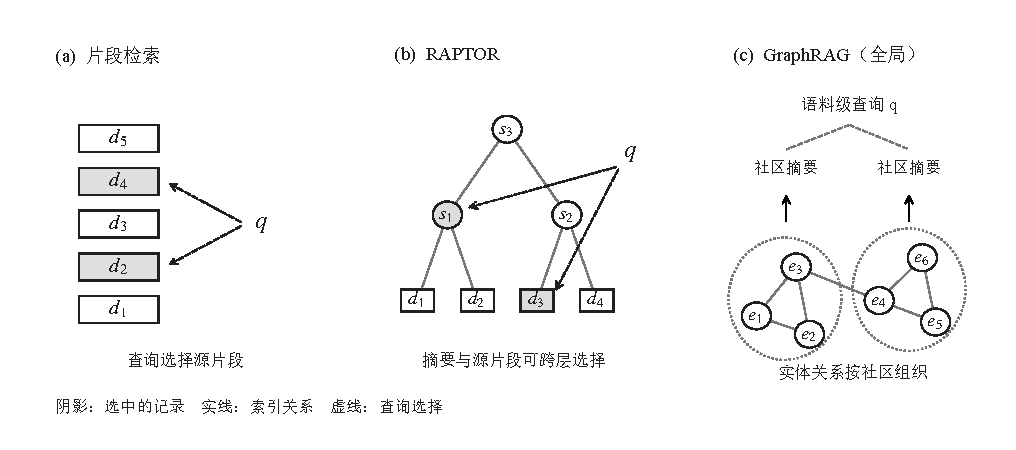
\includegraphics[width=\textwidth]{figures/review-knowledge-memory.pdf}
\caption{外部知识与研究记忆的组织方式。左、中两部分分别根据RAG、RAPTOR及GraphRAG的机制绘制\cite{rag,raptor,graphrag}；
右部综合MemGPT、Reflexion与科研状态管理需求\cite{memgpt,reflexion}，为本文分析示意，不代表原方法使用了完全相同的状态字段。各结构不按存储量或性能比例绘制。}
\label{fig:knowledge}\end{figure*}

\subsection{检索决策与证据支持}
除索引结构外，检索何时发生、结果如何被筛选，同样影响生成质量。
Self-RAG使用经过训练的反思标记，控制是否检索，并评价材料相关性、生成内容的支持程度及回答质量\cite{selfrag}。
与固定返回若干片段的流程相比，这一路线把检索需求和证据使用纳入生成决策。
它也说明“反思”可以具有不同技术含义：Self-RAG包含专门训练和控制标记，
并不是在任意模型之后添加一句检查提示就能获得相同机制。

面向科研的证据使用还需要区分相关、支持与充分三个层次。
某段文字可以与问题相关，却只讨论另一种数据设置；即使支持一个局部命题，也未必足以支持更广泛结论。
因此，检索输出需要保留对象、实验条件和结论范围，生成阶段则应维持这些限定。
在检索结果互相矛盾时，较合理的输出是呈现差异及其可能来源，而非强行综合成一致意见。
这一要求使科研RAG更接近文献分析过程，而不仅是为回答补充背景材料。

扩大上下文窗口可以减少部分切分与多次检索的需要，但不能完全代替上述过程。
Lost in the Middle显示，在所测模型和任务中，相关信息的位置会影响长上下文利用效果\cite{middle}。
这一发现不应机械外推到所有新模型，却说明上下文容量与有效信息利用需要分别评估。
在实际系统中，长上下文、检索筛选和多轮核查可以互补；方法选择应结合资料规模、查询类型及允许的调用预算。

\subsection{经历记忆、反思与分层存储}
外部知识主要描述已有研究，任务记忆则保存项目进行过程中产生的观察、计划和判断。
Generative Agents通过记忆流、相关经历检索、反思与规划，展示了代理如何在较长时间内维持行为连续性\cite{generative}。
这一设计的重要启发是，历史信息不必全部进入当前上下文，而可以根据相关性、时间及重要程度有选择地调用。
但其评价主要针对社会行为的可信感，迁移到科研任务时，需要重新定义哪些经历值得保留，以及怎样处理后来出现的反证。

Reflexion将环境或评价器的反馈转化为语言反思，并保存在经历记忆中，用于改善后续尝试\cite{reflexion}。
它不通过更新模型权重完成适应，而是改变下一次行动所依据的上下文。
这使失败尝试能够成为后续计划的输入，适合程序调试和具有明确反馈的任务。
反思的有效性同时依赖反馈质量：如果评价器无法识别错误，文字总结可能只是把错误解释得更完整。
因此，反馈信号、反思过程和记忆写入规则需要作为相互关联的设计选择讨论。

MemGPT将上下文管理类比为分层存储，通过显式操作在当前窗口与外部存储之间调度信息\cite{memgpt}。
相较于持续扩展提示或反复压缩全部历史，分层设计能够把信息保留与当前访问分开。
这一机制主要解决容量与调度问题，是否形成可靠科研记录，还取决于存入了何种内容。
观察、解释和计划具有不同地位：实验得到的数值是观察，对数值的原因分析是解释，下一轮配置属于计划。
若三者在摘要中混合，后续代理就难以判断哪些内容已经测量、哪些仍待检验。

\subsection{知识与记忆的协同维护}
从技术实现看，知识与记忆都可以采用文本、向量或图表示，二者的核心差异在于来源和更新方式。
论文知识随着外部资料变化而更新，项目记忆则随着研究活动逐步积累。
将二者相连，有助于解释某次实验为何采用特定方案，也能在新的文献出现时识别需要复查的旧判断。
然而，无来源区分的统一文本库容易产生循环引用：代理先写入推测，后续又检索到该推测并把它当成外部支持。
因而，共享存储不应取消原始资料与派生解释之间的区别。

对科研任务而言，记忆质量更适合用关键判断能否被重建来衡量。
与研究方向变化、异常结果和结论修正有关的记录，应保留其条件与依据；
重复性的接口说明与常规状态则可以适度压缩。
这样既能控制上下文开销，也避免把所有历史等量保存。
表\ref{tab:knowledge}总结了主要路线的处理对象及适用边界。
综合来看，知识增强与记忆机制的共同趋势，是由单纯“增加可见文本”转向对信息粒度、来源和使用时机进行管理。

\begin{table*}[t]\centering\tabletext
\caption{知识增强与记忆机制的比较。外部知识组织和项目经历管理服务于不同目标，不作统一性能排名。}
\label{tab:knowledge}
\begin{tabularx}{\textwidth}{@{}>{\raggedright\arraybackslash}p{25mm}YYY@{}}\toprule
路线与代表方法 & 核心机制 & 主要适用任务 & 需要关注的限制\\\midrule
片段检索：RAG\cite{rag} & 根据查询检索相关文档或片段，条件化生成 & 事实查询、参数定位、材料更新 & 相似性不等于证据支持，多处条件可能被遗漏\\
层次检索：RAPTOR\cite{raptor} & 递归聚类与摘要，跨抽象层检索 & 长文理解、跨段综合 & 高层摘要压缩细节，需要保留回溯关系\\
图检索：GraphRAG\cite{graphrag} & 实体关系、社区及社区摘要 & 主题分析、全局信息综合 & 抽取误差、实体歧义与索引维护成本\\
自适应检索：Self-RAG\cite{selfrag} & 训练反思标记，控制检索并评价生成支持 & 按需检索、事实性与引用改进 & 依赖训练与评价设计，不能等同于一般提示反思\\
经历与反思记忆\cite{generative,reflexion} & 检索历史经历，将反馈写入后续上下文 & 长期规划、重复尝试与错误修正 & 反馈失真可能固化错误，原始观察与解释需区分\\
分层存储：MemGPT\cite{memgpt} & 在当前窗口和外部存储间调度 & 长对话、持续任务与信息保留 & 信息可访问性与记录真实性需要分别检验\\\bottomrule
\end{tabularx}\end{table*}
